% ---------------------------------------------------------------- 6 experiments
\section{Experiments}\label{sec:exp}

\paragraph{Training.} The model (0.86M parameters) is first trained on 2{,}000 tube renders
(plain and wood backgrounds only) for 14 epochs. It is then fine-tuned on 3{,}000
renders, 60\% of them in broader styles: outlined and hollow ribbons, textbook
diagrams with gaps, rope twist, shaded tubes, multicoloured links and widths of
5--32\,px. Torus, Lissajous and random Fourier curves are added to braid closures.
Finally the full-resolution ridge branch is trained for 4 epochs on the frozen
trunk. The full recipe takes about 2.5 hours on two CPU cores; we report three seeds.

\begin{table*}[t]
\centering\small
\setlength{\tabcolsep}{\widetabcolsep}
\fittable{../tables/main}
\caption{\textbf{Main results on \bench{}} (\VthreeImages{} photo-like images of
\VthreeCables{} cables; unseen = backgrounds S3/S4). Crossing precision (P) and recall (R),
\ou{} (O/U) accuracy on matched crossings, fraction of images answered, and wrong
answers. Our full model recovers \VthreeRecall{} of crossings and answers
\VthreeCov\% of images with \VthreeWrong{} wrong answers.}
\label{tab:main}
\end{table*}

\paragraph{Main results.} \Cref{tab:main} compares label prediction, a classical parser and
our formulation with three dense networks, all trained on the same renders. The 250-class
classifier has median top-class probability 0.007; forced to answer it is right on
\ClfBenchAcc\% of images, and at $p\ge0.95$ it answers none. The skeleton parser misses
most crossings and reads \ou{} at chance; without the Euler gate it gives
\BaseWrongNoGate{} wrong answers. A U-Net that only segments finds crossings as well as any
model (precision \USegPrec, recall \USegRecall) yet names nothing: without \ou{} evidence no
type reaches probability 0.95. Detecting crossings is not the hard part; reading \ou{} is.
With \ou{} heads, both backbones read crossings and \ou{} almost perfectly and make no wrong
call. The U-Net pair answers more (\UPCov\% vs \VthreeCov\%), most clearly on unseen
backgrounds (\UPUnseenCov\% vs \VthreeUnseenCov\%). It has 3.6 times the parameters and was
trained in one stage on the broader styles, while the NanoTransformer was first trained on
plain tube renders; a size-matched comparison is left open. Per-session results are in the
supplement.

\begin{table*}[t]
\centering\footnotesize
\setlength{\tabcolsep}{\widetabcolsep}
\fittable{../tables/beatunet}
\caption{\textbf{Matched comparison with the U-Net pair.} Same data (3{,}000 renders), same one-stage
recipe (12 epochs), same device (Apple GPU), and the same parser (with the clutter filter).
Mean$\pm$sd over three seeds; wrong answers are summed over seeds. Blind v2 has 312 images, real 166.}
\label{tab:beatunet}
\end{table*}

\paragraph{Beating the U-Net pair.} The U-Net pair's lead over the NanoTransformer does not come from
crossings or \ou{}, which both read almost perfectly on the benchmark. It comes from the dense path. On
cluttered backgrounds the NanoTransformer's centre-line and mask fire on background texture
(\cref{sec:method}). We therefore compare three models on equal terms (\cref{tab:beatunet}): the U-Net
pair, the NanoTransformer widened to the same size and trained in one stage, and the UNetFormer. The
widened NanoTransformer stays far behind (\BUNanoVtwo{} correct on blind v2), so size and training
recipe do not explain the gap. The UNetFormer answers more blind-v2 images correctly than the U-Net
pair at every seed (\BUUfVtwoDiffs; \BUUfVtwo{} vs \BUUnetVtwo{} on average). It also answers more real
pictures (\BUUfRealDiffs; \BUUfReal{} vs \BUUnetReal). Image by image, \BUVtwoOnlyUf{} blind-v2 readings
are correct only for the UNetFormer and \BUVtwoOnlyUnet{} only for the U-Net pair, summed over seeds
(exact McNemar $p=\BUVtwoSeedP$ per seed). On real pictures the split is \BURealOnlyUf{} vs
\BURealOnlyUnet. Wrong answers barely change: \BUUfVtwoWrong{} vs \BUUnetVtwoWrong{} on blind v2 over
three seeds, all of them the same drawing of 9\_25 read as 3\_1\,\#\,4\_1 by both models. On the
real pictures every error is on one picture, which the set holds twice: a single strand with three figure-eight lobes,
read as 4\_1\,\#\,4\_1\,\#\,4\_1 while its folder label is 4\_1. On the benchmark the U-Net pair keeps a
small edge (\BUUnetBench\% vs \BUUfBench\% answered, no wrong answer for either). On unseen
backgrounds the per-seed difference is \BUUfUnseenDiffs{} points. The clDice topology
loss~\cite{shit2021cldice} trades part of the UNetFormer's blind and real gain for benchmark coverage
(\BUTopoBench\%; \BUTopoVtwo{} correct on blind v2). The centre-line was not breaking, so a loss
against breaks was not the missing piece.

\begin{table}[t]
\centering\footnotesize
\setlength{\tabcolsep}{3pt}
\fittable{../tables/ablation}
\caption{\textbf{Ablations} on \bench{} (v3 trunk unless noted). Silh.\ ans.\ =
fraction of silhouettes answered, which must be 0 because \ou{} is not visible.}
\label{tab:ablation}
\end{table}

\paragraph{Ablations.} \Cref{tab:ablation} isolates the parser's components.
\begin{itemize}
\item \textbf{Skeleton source.} Coverage comes from the skeleton source. Mask, then
  128-grid ridge, then 256-grid ridge, then both ridges gives 52, 62, 68 and 69\%
  answered, and 31, 28, 39 and 40\% on unseen backgrounds.
\item \textbf{Test-time views.} Without them, the model answers \NoTTASilCov\% of
  silhouettes, \NoTTASilWrong{} of them wrongly: from one view it commits to an
  \ou{} reading it cannot see. Averaging the views without the consistency shrink
  ($\gamma=0$) is worse: \GzeroSilCov\% of silhouettes answered, \GzeroSilWrong{} wrongly.
  The shrink, not the averaging, is what makes the system abstain.
\item \textbf{FFT input channel and seeds.} Three seeds of the full recipe give
  \SeedCov$\pm$\SeedCovSd\% answered (\SeedUnseen$\pm$\SeedUnseenSd\% on unseen backgrounds) and
  \SeedWrong{} wrong answers in total. Retrained without the FFT channel (one seed) the model
  answers \NoFFTCov\% (\NoFFTUnseen\% unseen): slightly lower, but within about two standard
  deviations of the seed spread, so we do not claim a benefit from the channel.
\item \textbf{Clutter filter.} Removing open centre-line pieces that carry no crossing raises the frozen
  model's answered fraction from \VthreeCov\% to 82\% (unseen backgrounds 40\% to 68\%) and the CPU-trained
  U-Net pair's from 86\% to 92\%, with no new wrong answers. The filter was designed after inspecting the
  benchmark's unseen-background failures and checked on 80 new renders in those styles, so its benchmark
  gain is not blind. On blind v2 it changes the frozen model by 0 images and the U-Net pair by 1.
\item \textbf{Euler gate.} On renders the gate changes nothing for our model, since
  the other checks already catch its few misses. For the skeleton parser it removes
  all \BaseWrongNoGate{} wrong answers. We keep it as a network-independent safety
  net for real images, where detection is weaker.
\end{itemize}

\begin{figure}[t]
\centering
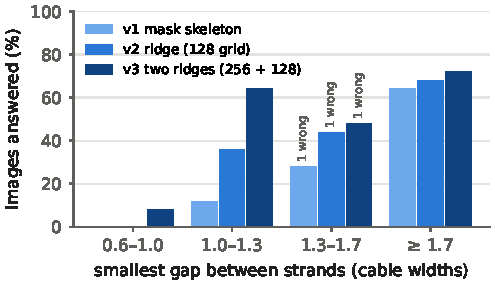
\includegraphics[width=\linewidth]{../figures/close_strands.pdf}
\caption{\textbf{Coverage as strands come closer} (100 images, 25 per bin). The
full-resolution centre-line head keeps strands apart down to about one \cw{}.
Below that, the strands touch and the system abstains. The single wrong answer
(same image in every version) is a 2.7\,px double crossing that no single view resolves.}
\label{fig:close}
\end{figure}

\paragraph{Strands that touch.} Abstentions on \bench{} come mostly from places where
two strands pass within a \cw{}. Their masks merge, the mask skeleton grows a false
branch, and the face between them disappears from the Euler count. Detection and
\ou{} are not the problem: crossing recall stays 0.93--0.97 and \ou{} accuracy
0.98--1.00 in every bin. \Cref{fig:close} shows that the
ridge skeleton raises overall coverage on the stress set from \CloseCovVone\% to
\CloseCovVthree\%. At 1.0--1.3 \cw s it rises from \CloseMidVone\% to \CloseMidVthree\%.
Below one \cw{} it reaches only \CloseLowVthree\%: there the strands touch, and
abstaining (and asking for another view) is the intended behaviour.

\begin{table}[t]
\centering\small
\setlength{\tabcolsep}{4pt}
\fittable{../tables/real}
\caption{\textbf{Real knot pictures answered} (166 public images, labelled by type
only); wrong answers in brackets. Traverser = skeleton parser.}
\label{tab:real}
\end{table}

\paragraph{Real pictures.} On 166 real knot pictures (\cref{tab:real}), the skeleton
parser answers none. Our model answers \RealVoneAns{} before and \RealAns{} after the
broader styles, all correct. Answers come from drawings and renders. None of the
\RealPhotoN{} photographs of physical objects (rope, cord, sculpture) is answered:
their textures still break the skeleton. The training styles were chosen after
inspecting four failures from this set, so these numbers are not a blind test.
\todo{Add a blind real set and the annotated real cable photographs.}

\begin{table}[t]
\centering\footnotesize
\setlength{\tabcolsep}{3pt}
\fittable{../tables/blind}
\caption{\textbf{Blind set}, scored once with the frozen model (\BlindN{} images from sources
never used or viewed during development: knotR drawings and POV-Ray renders of KnotPlot
centrelines). Correct = same type up to mirror image.}
\label{tab:blind}
\end{table}

\paragraph{Blind evaluation.} Before scoring, the NanoTransformer and its parser settings were
frozen by hash, and the set was built without viewing any image (\cref{tab:blind}). Renders behave like
the benchmark: \BlindRendAns{} of \BlindRendN{} answered, \BlindRendWrong{} wrong. Drawings expose a
failure mode the benchmark never showed: \BlindDrawAns{} of \BlindDrawN{} answered and
\BlindDrawWrong{} wrong (\cref{fig:blindfail}). In each of them the under-strand gap is one or two
pixels wide, every crossing is read with probability 0.96--0.99, and all eight test-time views agree
on the reading. View agreement detects evidence that depends on the view (a silhouette), not
evidence that is consistently misread. A network-independent check of the intensity break at each
crossing is the obvious next gate; it must be evaluated on a new blind set.

\begin{figure*}[t]
\centering
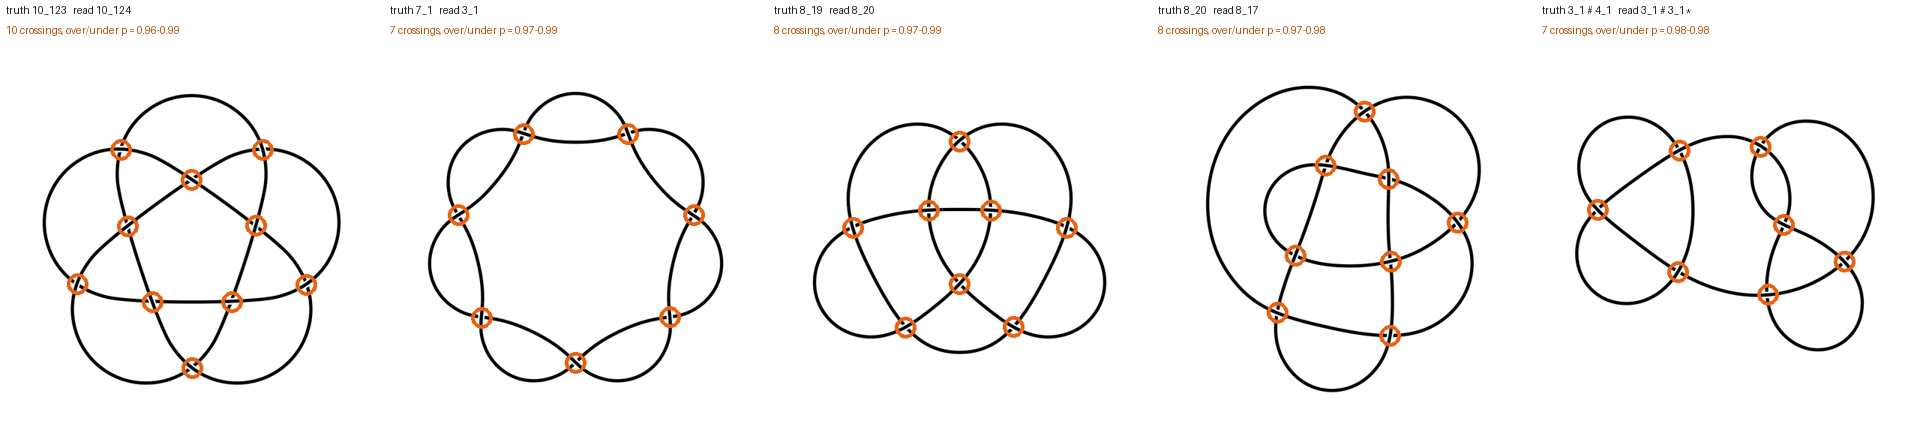
\includegraphics[width=\linewidth]{../figures/blind_failures.png}
\caption{\textbf{All wrong answers on the blind set} (post-scoring analysis). Orange circles: detected
crossings. Gaps at the under-strands are one or two pixels wide; the model reads \ou{} with
probability 0.96--0.99 at every crossing and all test-time views agree.}
\label{fig:blindfail}
\end{figure*}

\paragraph{Baselines on the blind set.} The U-Net pair, scored once as a baseline, answers
\UPBlindAns{} images, \UPBlindCorrect{} correctly; \UPBlindWrong{} of its answers are wrong,
\UPBlindDrawWrong{} of them on drawings with nearly invisible gaps, the same failure as the
frozen model. The classifier is right on \ClfBlindAcc\% of the blind set (and on \ClfTrainAcc\%
of the real pictures it was trained on).

\begin{table*}[t]
\centering\footnotesize
\setlength{\tabcolsep}{\widetabcolsep}
\fittable{../tables/minkowski}
\caption{\textbf{Minkowski attention, the Lebesgue loss and gap evidence.} Mean$\pm$sd over seeds;
wrong answers are summed over seeds. Variants are added cumulatively (\cref{sec:method}). A seed
fixes the data order and augmentation, so each variant has a plain counterpart with the same seed
(see text). $^\dagger$Blind v1 is no longer blind for the gap evidence, whose design followed its
errors. Blind v2 is (\cref{tab:blind2}).}
\label{tab:minkowski}
\end{table*}

\paragraph{Minkowski attention and the Lebesgue loss.} Each variant was trained with the full recipe
(\cref{tab:minkowski}). The content-attention variant has three CPU seeds: 0 and 1 on the machine that
trained the plain model, and 2 on a laptop CPU. All three variants also have three seeds trained on
an Apple GPU. A seed fixes the data order and augmentation, so we compare each variant with the
plain model of the same seed. Against it, Minkowski content attention changes the answered fraction
on unseen backgrounds by \MkCpuUnseenDiffs{} points on CPU, and the number of correct blind-v2
images by \MkCpuVtwoDiffs{}. It makes one more wrong blind-v2 answer over the three seeds (3 vs 2).
No paired comparison goes the other way. On the GPU the
differences are larger (\MkMpsUnseenDiffs{} points; \MkMpsVtwoDiffs{} images). However, the plain
model was never trained on the GPU, and the Lebesgue loss alone, which has no Minkowski component,
gains about as much there (\LebMpsUnseenDiffs{} points). The GPU rows therefore mix the device with the
model. On CPU at seed 0, the Lebesgue loss alone loses 5 points on unseen backgrounds and the
position bias gains 3. On the 166 real pictures there is no consistent change (\MkCpuRealDiffs{}).
No model makes a wrong benchmark call. On the close-strands set the variant makes 4 wrong answers over
three seeds, against 3 for the plain model. The learned exponents
stay Euclidean: $p\in[\LearnedPmin,\LearnedPmax]$ in every head of all \LearnedModels{} trained
models, and the slopes stay near their initial values (\LearnedAlphaMin--\LearnedAlphaMax). Whatever
helps is a multi-scale locality prior on the token grid, not a non-Euclidean neighbourhood. Seeds
alone move blind-v2 by up to three images (\PlainVtwoMin--\PlainVtwoMax{} correct for the plain
model). Three paired seeds give a consistent direction (benchmark coverage and blind v2 up, wrong
answers unchanged), not a precise effect size. The variants stay well behind the U-Net pair.

\begin{table}[t]
\centering\footnotesize
\setlength{\tabcolsep}{3pt}
\fittable{../tables/blind2}
\caption{\textbf{Blind set v2} (\VtwoN{} images, frozen before any model or setting in this
table was scored on it, never viewed: \VtwoDrawN{} line drawings with halo gaps of 0.1--0.8 line
widths, \VtwoRendN{} POV-Ray renders from new viewpoints). Correct = same type up to mirror image.}
\label{tab:blind2}
\end{table}

\paragraph{Gap evidence and a second blind set.} Blind v1 can no longer test a remedy for its own
failures, because they were inspected. We therefore froze a second blind set
(\cref{tab:blind2}) before scoring the gap evidence or any new model on it. Its drawings come
from a renderer used nowhere in training, with gaps from clear to nearly invisible. Its renders
show the v1 curves from new directions, which gives new diagrams. The three plain seeds answer
\PlainVtwoMin--\PlainVtwoMax{} images correctly (mean \PlainVtwoCorrect). With the gap evidence,
the frozen network answers \GapVtwoCorrect{} correctly (\FrozenVtwoCorrect{} without it) with
\GapVtwoWrong{} wrong answer, as before. The gain comes from drawings (\FrozenVtwoDrawCorrect{}
$\to$ \GapVtwoDrawCorrect{} correct). On the benchmark, the close-strands set and the real pictures,
nothing changes (\cref{tab:minkowski}). On development images the evidence improves the
log-likelihood of the network's \ou{} readings from \GapLLnone{} to \GapLLedge{} and adds one
answer (\GapDevNoCheckAns{} $\to$ \GapDevAns{}, no wrong). A veto rule ($p\to\frac12$ when $D$ is
small) instead removes correct answers (\GapVetoAns{} answered) and was not adopted.

Two caveats. First, a cross-section measure (correlation of the strand's profile with its free
profile) fits the development crossings better (log-likelihood \GapLLxsec). But on the shaded 3D
renders of the real-picture set it has the wrong sign at most crossings the network reads correctly
(all seven on one 7\_1 render), and it cost six correct answers there. We chose the edge measure after seeing this, so the
real-picture numbers for the gap evidence are not blind. Blind v2 was frozen before that choice
was scored. Second, the effect is small: three answers out of \VtwoN{}, just above the
seed-to-seed range. On blind v1 (post hoc) the evidence adds six correct answers and one
wrong, and the original five errors remain: they are not \ou{} errors alone, as 7\_1 read as
3\_1 shows. The U-Net pair is far stronger on v2 (\UPVtwoCorrect{} correct of \UPVtwoAns{}
answered, \UPVtwoWrong{} wrong), as on every other set.

\paragraph{Runtime.} On four CPU threads of a laptop (Apple silicon, PyTorch on CPU), the median
image takes 0.54\,s in the network with eight test-time views (0.08\,s with one) and 0.35\,s in the
parser, including both skeleton sources and the gap measure: 0.9\,s in total (20 benchmark images).

\begin{figure*}[t]
\centering
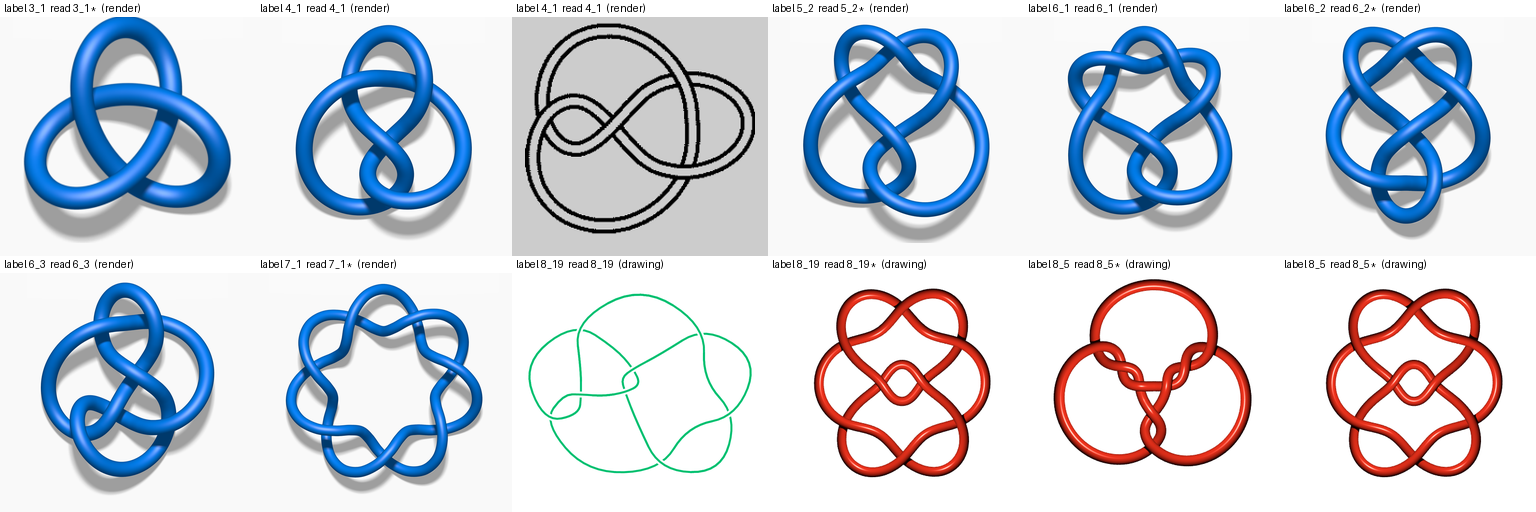
\includegraphics[width=\linewidth]{../figures/real_answered.png}
\caption{\textbf{All \RealAns{} real pictures our system answers}, each correct (up to
mirror image, marked $*$). Every answer comes from a drawing or a render; none of the
photographs of physical objects is answered.}
\label{fig:real}
\end{figure*}
